\documentclass[11pt]{article}
\usepackage[T1]{fontenc}
\usepackage[utf8]{inputenc}
\usepackage{lmodern}
\usepackage[margin=1in]{geometry}
\usepackage{amsmath,amssymb,mathtools}
\usepackage{booktabs,longtable,array}
\usepackage{fancyvrb}
\usepackage[hidelinks]{hyperref}
\usepackage{microtype}
\usepackage{graphicx}
\usepackage{adjustbox}
\pdfinfoomitdate=1
\pdftrailerid{}
\pdfsuppressptexinfo=15
\setlength{\parindent}{0pt}
\setlength{\parskip}{0.6em}
\setlength{\emergencystretch}{3em}
\renewcommand{\arraystretch}{1.25}
\setlength{\tabcolsep}{4pt}
\sloppy
\graphicspath{{Revision/universe_model/}}
\title{UM-1: an accurate approximate solution of the coupled field equations}
\author{dirac16complex project (with Claude Opus 5.5)}
\date{}
\begin{document}
\maketitle
\tableofcontents
\newpage

Version 1 of 2026-10-17, step [4] of the author's order of 2026-10-17, with the author's correction: "use Kohn-Sham theory for the dirac16complex field, which couples to all other fields". The model is defined in \texttt{MODEL.\allowbreak{}md}, its field equations are derived in \texttt{FIELD\_\allowbreak{}EQUATIONS.\allowbreak{}md}, and the origin of every ingredient is in \texttt{PROVENANCE.\allowbreak{}md}. The scripts are in \texttt{solution/\allowbreak{}} and every number in this document comes from them. The tables of section 9 are generated by \texttt{solution/\allowbreak{}solve\_\allowbreak{}model.\allowbreak{}py} from the outputs of the run, and the checks are in \texttt{solution/\allowbreak{}reports/\allowbreak{}solution-{}\allowbreak{}checks.\allowbreak{}json}. The labels are those of \texttt{MODEL.\allowbreak{}md}: DERIVED, TAKEN, STANDARD, ASSUMED, INVENTED, OPEN. A change to the model that the solution forces is labelled CHANGED.

Coordinates are the author's: $X = \{x_0, x_1, \dots, x_7\}$. $x_0$ is the hidden space-like direction, $z = 6Hx_0$ is real and $y = \ln|\sin z|/(6H) \in [-L, 0]$ (with $(\sin^2 z)^{1/6}$ on the positive branch); $x_1, x_2, x_3$ are 3-space, $x_4$ is the time and $x_5, x_6, x_7$ are the extra times. The block $(x_0, x_5, x_6, x_7)$ has the scale factor $f = e^{-a_4}b_4^{1/2}$ and the rate $h_4 = \dot f/f$. Here $k = e^{2a_4}/b_4 = 1/f^2$, $A = \dot a_4$ is the four-dimensional Hubble rate, and the Lovelock weights are $\alpha_k = w_kH^{2-2k}$.

\section*{1. Summary of the results}
\addcontentsline{toc}{section}{1. Summary of the results}

\begin{enumerate}
\item The solution is a hierarchy of approximations in small parameters (section 2): the bookkeeping parameter $\epsilon$ of the metric series, $(A/H)^2$ (the late-time expansion rate against the cell scale, $4\times10^{-93}$ today), $\kappa\rho/H^2$ (the sources against the cell curvature) and the portal amplitudes. At each order the field equations become ordinary equations or eigenproblems, which are solved numerically with stated errors.
\item Gravity (section 3, DERIVED, \texttt{solution/\allowbreak{}vacua.\allowbreak{}py}). On the static-block slicing ($h_4 = 0$) the x4 constraint reads $3G(k)A^2 = \Lambda_{eff} + \kappa\rho$, with the effective-Newton factor $G(k) = 1 - 24w_2k + 72w_3k^2$. For every set of weights, the only static vacuum without sources is $k_0 = 1/(4w_2)$, $\Lambda_0 = -3H^2/(4w_2)$. A theorem of the homogeneous reduction: the block mode about that vacuum has $\lambda^2 = k_0G(k_0)H^2/4$. Attractive four-dimensional gravity therefore comes with an exponentially unstable block, and a stable block comes with repulsive gravity.
\begin{itemize}
\item The author's weights $(1, 1/32, 1/1152)$ give $G(k_0) = -1$: repulsive gravity.
\item The author's $\Lambda = -10H^2$ admits no static block with a small cosmological term.
\item UM-1 is therefore CHANGED to the benchmark weights $(1, 1/32, 1/768)$, which give $G(k_0) = +1$, and to $\Lambda = -24H^2 + \delta\Lambda$. A block stabiliser with $\Delta m^2 > 2H^2$ is ASSUMED; its origin is OPEN.
\item Near the vacuum the block tracks $\delta k = (\kappa p_0 - \delta\Lambda - 12A^2)/(3H^2)$. The extra times therefore keep deflating, slowly ($h_4 = 4A\dot A/(k_0H^2) < 0$), and are never static.
\end{itemize}
\item Masses (section 4, DERIVED, \texttt{solution/\allowbreak{}masses.\allowbreak{}py}).
\begin{itemize}
\item The photon, gluon and graviton are exactly massless.
\item The W and Z masses come from the Higgsless tip. A positive tip term gives at most $m_W = 0.01824\,m_{KK}$.
\item The Kaluza-Klein scale is fitted to the measured $\rho_0 - 1$: $m_{KK} = 121$ TeV, which gives $H = 23.4$ TeV and an $x_0$ period $\pi/(6H) = 4.4\times10^{-21}$ m.
\item The electron, up, down and neutrino masses come from chiral zero modes with $c_f = f\mu_fL \approx 10$ to $19.5$.
\item The uncertainty estimate $\hbar c/(2\Delta s)$ exceeds every fermion mass by a factor $5\times10^{7}$ to $10^{16}$. Chiral zero modes are the exception to the author's Heisenberg argument; the W mass, too, comes 99.9 \% from the tip.
\end{itemize}
\item dirac16complex, Kohn-Sham, coupled to all fields (section 5, DERIVED, \texttt{solution/\allowbreak{}ks\_\allowbreak{}coupled.\allowbreak{}py}).
\begin{itemize}
\item At the vacuum slice the fold band is massless ($\varepsilon = \kappa|k|$ exactly, $g_F = 8$ states per 3-momentum).
\item The lightest odd-parity bulk level, $2.17492\,m = 50.9$ TeV, is the dark matter.
\item The portal mean fields of the Standard-Model fermions shift the dark-matter level linearly. They leave the fold band massless and pass the Hellmann-Feynman and y-exchange checks.
\item The coupled fixed point $\Psi \leftrightarrow$ Standard Model $\leftrightarrow$ block converges.
\end{itemize}
\item Cosmology (section 6, DERIVED, \texttt{solution/\allowbreak{}cosmology.\allowbreak{}py}).
\begin{itemize}
\item UM-1 has ONE generation (the author's particle list), so its Standard-Model $N_{eff}$ is 1.015. The $\Psi$ fold band must supply $\Delta N_{eff} \approx 2$.
\item That requires $\Psi$ to decouple from the plasma at $g_{*s} = 12.3$, i.e. in the QCD crossover. Decoupling above it gives $N_{eff} = 1.30$ to $1.37$, excluded by about $10\sigma$; decoupling in the pion gas gives $3.54$ ($+3.2\sigma$).
\item With $N_{eff} = 2.99$ and $\theta_*$ fixed, $H_0 = 66.75$ km/s/Mpc and $r_{drag} = 147.4$ Mpc. The eBOSS DR16 BAO give $\chi^2 = 11.6$ for 12 points (Planck $\Lambda$CDM: 10.2).
\item The CNB has $T_\nu = (4/11)^{1/3}T_{CMB} = 1.945$ K.
\end{itemize}
\item Conflicts with data, stated plainly (section 7).
\begin{itemize}
\item There is no Higgs boson, while one is observed at 125 GeV.
\item Without a Higgs, $WW$ scattering violates perturbative unitarity near 1.2 TeV, far below $m_{KK}$.
\item One generation needs the tuned decoupling of item 5.
\item The cosmological term needs $\delta\Lambda/H^2 \approx 8\times10^{-93}$.
\end{itemize}
\end{enumerate}

\section*{2. The approximation scheme}
\addcontentsline{toc}{section}{2. The approximation scheme}

The coupled system of \texttt{FIELD\_\allowbreak{}EQUATIONS.\allowbreak{}md} section 9 is solved as a series in four small parameters. Each is computed below, not assumed:

\begin{longtable}{>{\raggedright\arraybackslash}p{0.182\linewidth}>{\raggedright\arraybackslash}p{0.318\linewidth}>{\raggedright\arraybackslash}p{0.368\linewidth}}
\toprule
\textbf{parameter} & \textbf{meaning} & \textbf{size in the solution} \\
\midrule
$\epsilon$ & metric perturbations (CMB anisotropy) & $10^{-5}$ (STANDARD) \\
$(A/H)^2$ & late-time expansion rate against the cell scale & $3.7\times10^{-93}$ today \\
$\kappa\rho/H^2$, $\kappa p_0/H^2$ & sources against the cell curvature & of order $(A/H)^2$ (the Friedmann equation) \\
$e_V, e_D, e_S$ & portal mean fields against $m$ & proportional to the Standard-Model densities in units of $m^3$ \\
\bottomrule
\end{longtable}

\begin{itemize}
\item Order 0 in all of them: the static block vacuum (section 3), the $x_0$ eigenproblems of every field on the vacuum cell (section 4), and the Kohn-Sham ground state of $\Psi$ on the vacuum cell (section 5).
\item First order in $(A/H)^2$ and $\kappa\rho/H^2$: the four-dimensional Friedmann equation with $G_{eff} = G/G(k_0)$, and the quasi-static block shift that makes the extra times keep deflating (section 3.4).
\item First order in the portal amplitudes: the linear response of the Kohn-Sham state of $\Psi$ (section 5.3). It feeds back on the Standard-Model masses and on the block through the hidden pressure $p_0$ (section 5.5).
\item First order in $\epsilon$: the acoustic physics of the CMB and the BAO in the four-dimensional effective theory. It uses the standard fitting formulae, calibrated once on Planck $\Lambda$CDM (section 6). Its accuracy is set by the fitting formulae, a few parts in $10^4$ on $\theta_*$ and $r_{drag}$.
\end{itemize}

\section*{3. Gravity: the Einstein-Lovelock vacuum and the block}
\addcontentsline{toc}{section}{3. Gravity: the Einstein-Lovelock vacuum and the block}

\subsection*{3.1 The static-block slicing (exact)}
\addcontentsline{toc}{subsection}{3.1 The static-block slicing (exact)}

With $\dot a_4 = A$, $\ddot a_4 = 0$, $u = 2A$ (so $h_4 = 0$ and $k$ constant) and $\dot u = 0$, the record's three background components (\texttt{Revision/\allowbreak{}field\_\allowbreak{}equations\_\allowbreak{}a4/\allowbreak{}a4-{}\allowbreak{}equations.\allowbreak{}json}, generalSource) are, for general $w_2, w_3$ (check V1):

\[F_4 = -3G(k)A^2 + 6H^2k(1 - 2w_2k) + \Lambda + \kappa\rho,\qquad G(k) = 1 - 24w_2k + 72w_3k^2\]

\[F_0 = 6(12w_2k - 1)A^2 - 12(w_2 - 18w_3k)A^4/H^2 + 3H^2k + \Lambda - \kappa p_0\]

$F_1$ is $F_4$ with $-\kappa p_3$ in place of $\kappa\rho$. In Einstein gravity ($w_2 = w_3 = 0$), $F_4 = 0$ is the Friedmann equation $3A^2 = \Lambda + 6H^2k + \kappa\rho$. $G(k)$ is therefore the ratio of the effective four-dimensional Newton constant to the Einstein one. $G > 0$ means attractive gravity; $G < 0$ means a negative Newton constant, i.e. matter decelerates the expansion in the wrong direction.

\subsection*{3.2 The static vacuum and the effective Newton constant}
\addcontentsline{toc}{subsection}{3.2 The static vacuum and the effective Newton constant}

$F_4 = F_0 = 0$ with $A = \rho = p_0 = 0$ has exactly one solution with $k \neq 0$ (check V2):

\[\adjustbox{max width=\linewidth}{$\displaystyle k_0 = \frac{1}{4w_2},\qquad \Lambda_0 = -\frac{3H^2}{4w_2},\qquad G(k_0) = -5 + \frac{9w_3}{2w_2^2} .$}\]

\begin{itemize}
\item The author's weights $w = (1, 1/32, 1/1152)$ give $k_0 = 8$, $\Lambda_0 = -24H^2$ and $G(k_0) = -1$: REPULSIVE gravity in the only static vacuum. With these weights, $G(k) > 0$ only for $k < 6 - 2\sqrt5 = 1.528$ or $k > 6 + 2\sqrt5 = 10.47$.
\item The author's $\Lambda = -10H^2$: the hidden component gives the quasi-static $k = 10/3$, where $\Lambda_{eff} = 35H^2/6$ and $G = -29/36$. That is a cosmological term of the size of the cell curvature, with repulsive gravity. No static vacuum with a small cosmological term exists for $\Lambda = -10H^2$.
\end{itemize}

\begin{figure}[htbp]
\centering
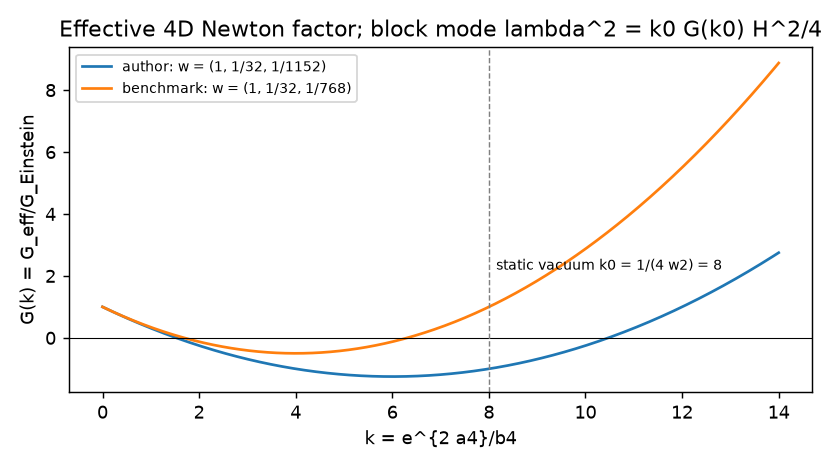
\includegraphics[width=0.85\linewidth]{solution/figures/fig1_newton_factor.png}
\caption{The effective Newton factor G(k) for the author's weights and the benchmark; the static vacuum k0 = 8.}
\end{figure}

\subsection*{3.3 The block mode: a theorem of the homogeneous reduction}
\addcontentsline{toc}{subsection}{3.3 The block mode: a theorem of the homogeneous reduction}

Linearising the $x_1$ and $x_0$ components (solved for $\ddot a_4$ and $\dot u$; the Jacobian has determinant $-24$) together with $\dot k = k(2\dot a_4 - u)$ about the vacuum gives, for general weights (check V3), the characteristic polynomial

\[\adjustbox{max width=\linewidth}{$\displaystyle \lambda\,\big(32w_2^3\lambda^2 + (10w_2^2 - 9w_3)H^2\big) = 0,\qquad \lambda^2 = \frac{k_0\,G(k_0)}{4}\,H^2 .$}\]

The linearised constraint vanishes identically, and the zero eigenvalue is the de Sitter direction ($u = 2\dot a_4$). So the block is stable (oscillating with $\omega^2 = -\lambda^2$) exactly when gravity is repulsive, and it is unstable (growing like $e^{\lambda x_4}$) exactly when gravity is attractive (check V4):

\begin{longtable}{>{\raggedright\arraybackslash}p{0.256\linewidth}>{\raggedright\arraybackslash}p{0.113\linewidth}>{\raggedright\arraybackslash}p{0.273\linewidth}>{\raggedright\arraybackslash}p{0.209\linewidth}}
\toprule
\textbf{weights} & \textbf{$G(k_0)$} & \textbf{4D gravity} & \textbf{block} \\
\midrule
author $(1, 1/32, 1/1152)$ & $-1$ & repulsive & stable, $\omega = \sqrt2H$ \\
benchmark $(1, 1/32, 1/768)$ & $+1$ & attractive (Einstein value) & unstable, $\lambda = \sqrt2H$ \\
\bottomrule
\end{longtable}

The instability has a natural reading in the author's picture. A static block is not where an attractive-gravity universe starts: it runs away from it at the rate $\lambda \sim H$. That is the exponential evolution of the extra times of the primordial era.

CHANGED (UM-1 version 1.1, forced by the solution):
\begin{itemize}
\item The cubic weight is $w_3 = 4w_2^2/3 = 1/768$, so that $G(k_0) = 1$ and the four-dimensional Newton constant has its Einstein value at the vacuum.
\item $\Lambda = \Lambda_0 + \delta\Lambda = -24H^2 + \delta\Lambda$.
\item A block stabiliser is ASSUMED: an additional potential for $k$ whose curvature exceeds $k_0G(k_0)H^2/4 = 2H^2$. The natural candidate is the renormalised Dirac-sea (Casimir) energy of $\Psi$ and of the Standard-Model fields in the cell as a function of $f$, which the Kohn-Sham record does not contain (it normal-orders the sea). Its computation is OPEN.
\end{itemize}

The radion then has a mass of order $H$ (tens of TeV). It mediates no long-range force, so the local and the cosmological Newton constants agree.

\subsection*{3.4 Slow deflation near the vacuum (the extra times are never static)}
\addcontentsline{toc}{subsection}{3.4 Slow deflation near the vacuum (the extra times are never static)}

To first order in $\delta k = k - k_0$, $\delta\Lambda$, $A^2$ and the sources, $\partial F_4/\partial k = 0$ at $k_0$. The constraint is therefore the Friedmann equation $3G(k_0)A^2 = \delta\Lambda + \kappa\rho$, and the hidden component gives the quasi-static block

\[\adjustbox{max width=\linewidth}{$\displaystyle \delta k = \frac{\kappa p_0 - \delta\Lambda - 12A^2}{3H^2},\qquad h_4 = -\frac{\dot k}{2k} = \frac{4A\dot A}{k_0H^2} < 0 \quad (\dot A < 0) .$}\]

The block keeps deflating as long as the universe decelerates or its Hubble rate falls: $f$ shrinks while $A$ falls. The rate is suppressed by $(A/H)^2$. With $\dot A = -(1+q)A^2$, the deflation today is $h_4/A = -4(1 + q_0)(A/H)^2/k_0 \approx -10^{-93}$ (section 9). The $x_0$-generated masses scale like $1/f$, so they drift by the same relative amount per Hubble time, far below every bound on varying constants. This keeps the binding statement "the extra times deflate exponentially, never static" in the primordial era. It is replaced by a slow, never-vanishing deflation in the late era (a labelled departure: a late exponential deflation at a rate of order $H$ would change the masses by order one per $10^{-28}$ s).

\section*{4. Masses from the $x_0$ wave functions}
\addcontentsline{toc}{section}{4. Masses from the $x_0$ wave functions}

\subsection*{4.1 Gauge fields and the graviton}
\addcontentsline{toc}{subsection}{4.1 Gauge fields and the graviton}

On each half of the cell, $t = y/L \in [-1, 0]$, the $x_0$ operator of a gauge field is $-e^{-3\eta t}(e^{3\eta t}u')' = \Lambda u$ with $\eta = HL$ and $\Lambda = (m\,fL)^2$. The fold condition is $u'(0) = 0$ and the tip (Robin) condition of the sigma field is $u'(-1) = \beta u(-1)$. Every solution is a function of $y(z) = \ln|\sin z|/(6H)$ and is therefore periodic in $x_0$ with period $\pi/(6H)$ (check M6).

\begin{itemize}
\item Unbroken generators ($\beta = 0$): $\Lambda_0 = 0$ (the photon, the gluons, and the graviton, whose zero mode is flat as well) and $\Lambda_n = 9\eta^2/4 + n^2\pi^2$ exactly (substitute $u = e^{-3\eta t/2}w$); the shooting solver reproduces these to $3\times10^{-13}$ (check M1). $m_{KK} = \sqrt{\Lambda_1}/(fL)$.
\item The Higgsless tip: a POSITIVE tip term (a positive $v_\Sigma^2$) cannot make the W heavier than the Dirichlet-tip level. That level satisfies $\tanh q = 2q/(3\eta)$, $\Lambda_D = 9\eta^2/4 - q^2 = 0.010016$ for $\eta = 3$ (check M2), so $m_W \leq 0.01824\,m_{KK}$ and $m_{KK} \geq 4.41$ TeV.
\item Custodial symmetry gives $c_{tip}(Z)/c_{tip}(W) = 1/\cos^2\theta_W$, so $\beta_Z = \beta_W/\cos^2\theta_W$. The saturation of $\Lambda(\beta)$ makes $\rho = m_W^2/(m_Z^2\cos^2\theta_W)$ larger than 1 by $5.6\times10^{-4}(100\,\text{TeV}/m_{KK})^2$. $m_{KK}$ is FITTED to the measured $\rho_0 - 1 = 0.00038 \pm 0.00020$: $m_{KK} = 121.2$ TeV, $H = 23.42$ TeV, proper half-cell $fL = 8.9\times10^{-21}$ m (check M4). With $m_W$ as input, the predicted $m_Z$ lies 0.017 GeV below the measured value (the on-shell angle; loop corrections of a Higgsless theory are not included).
\item The W mass is a tip effect. In the Rayleigh quotient of its eigenfunction the bulk hidden-momentum part is $1.3\times10^{-3}$ of $m_W^2$ and the tip part is the rest (check M3).
\end{itemize}

\begin{figure}[htbp]
\centering
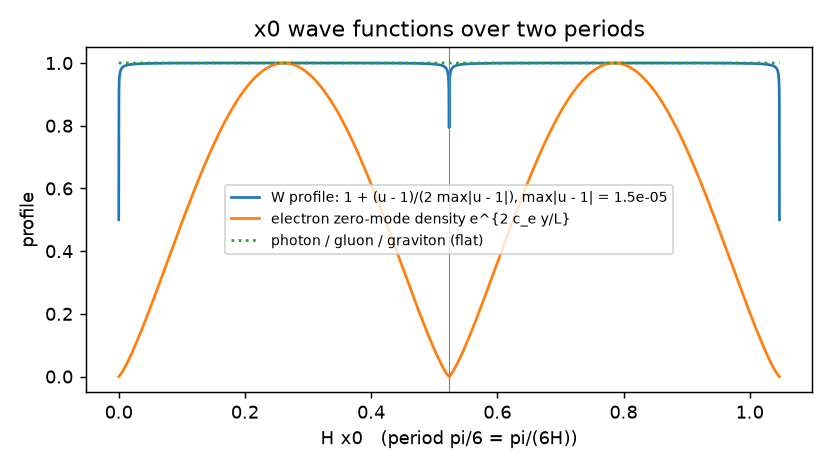
\includegraphics[width=0.85\linewidth]{solution/figures/fig2_x0_profiles.png}
\caption{The x0 wave functions over two periods: the W profile, the electron zero-mode density, the flat massless modes.}
\end{figure}

\begin{figure}[htbp]
\centering
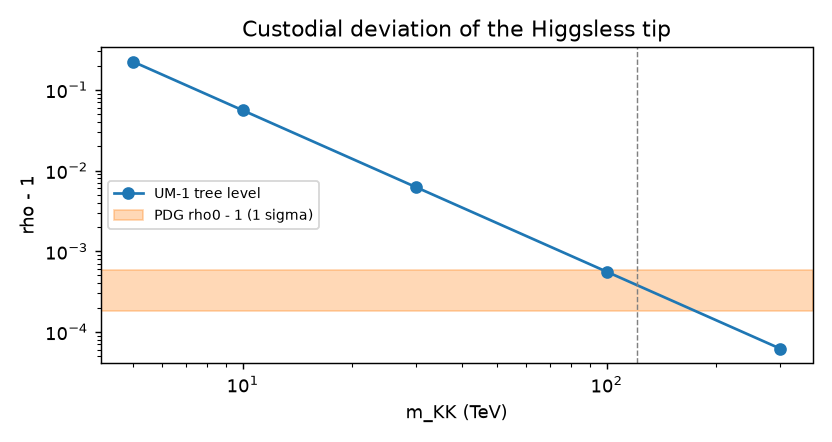
\includegraphics[width=0.85\linewidth]{solution/figures/fig3_rho.png}
\caption{The tree-level custodial deviation rho - 1 against m\_KK, with the measured band; the fitted m\_KK.}
\end{figure}

\subsection*{4.2 Fermions and the Heisenberg argument}
\addcontentsline{toc}{subsection}{4.2 Fermions and the Heisenberg argument}

Each fermion has a chiral zero mode $\chi = (e^{ct}, 0)$ with $c = f\mu_fL$ (\texttt{FIELD\_\allowbreak{}EQUATIONS.\allowbreak{}md} section 5). Its normalised tip value is $\zeta(c)^2 = 2ce^{-2c}/(1 - e^{-2c})$, and $m_f = \lambda_f m_{KK}\zeta(c_L)\zeta(c_R)$ (here $\lambda_f = 1$, $c_L = c_R = c_f$).
\begin{itemize}
\item $m_e$, $m_u$, $m_d$ and $m_\nu = 0.05$ eV (one generation; chosen at $\sqrt{\Delta m^2_{atm}}$) give $c_f$ between 10.4 and 19.5, i.e. bulk masses $\mu_f$ of 9.5 to 18.4 $H$ (check M5; section 9).
\item The profiles are localised at the fold, with proper widths $\Delta s \approx 10^{-22}$ m. The author's estimate $mc^2 \geq \hbar c/(2\Delta s)$ would give 220 to 430 TeV, while the actual masses are $2\times10^{-8}$ to $10^{-16}$ of that.
\item This is the DERIVED exception of \texttt{FIELD\_\allowbreak{}EQUATIONS.\allowbreak{}md} (check D3 there). The hidden momentum of a chiral zero mode is cancelled by its bulk mass ($h\chi = 0$), and its mass is set by its value at the tip, not by its localisation.
\item For bosons the Rayleigh quotient is the mean squared hidden momentum, and the uncertainty bound holds. But the W mass is dominated by the tip term (section 4.1), so here too the mass comes from the boundary, not from localisation.
\end{itemize}

\section*{5. dirac16complex: the Kohn-Sham solution coupled to all fields}
\addcontentsline{toc}{section}{5. dirac16complex: the Kohn-Sham solution coupled to all fields}

\subsection*{5.1 The equations and their implementation}
\addcontentsline{toc}{subsection}{5.1 The equations and their implementation}

The Kohn-Sham block of \texttt{FIELD\_\allowbreak{}EQUATIONS.\allowbreak{}md} section 6, with the portal mean fields of the Standard-Model fermions:

\[\adjustbox{max width=\linewidth}{$\displaystyle h_j = j\big[-(i/f)\sigma_1\partial_y + M_{eff}(y)\sigma_2 + \kappa|k|\sigma_3\big] + v_v(y),\qquad M_{eff} = m + \tfrac{15}{16}\lambda S + e_DP_{fold} + e_SP_{tip},\qquad v_v = -\tfrac{1}{16}\lambda n + e_VP_{fold}$}\]

\begin{itemize}
\item The fermion profiles: $P_{fold}(y) = e^{2c_ey/L}$ is the shape of the electron zero-mode density, with $c_e = 11.20$ from section 4 (the Standard-Model fermions sit at the fold). $P_{tip}$ is a unit-weight exponential of width 0.1 at $y = -L$, standing in for $\delta_{tip}$.
\item The portal amplitudes $e_V = g_V\sum_fq_fn_f$, $e_D = g_D\sum_fm_fs_f$ and $e_S = g_S\sum_fs_f$ (P1, P5, P2 of \texttt{MODEL.\allowbreak{}md}) are in units of $m$.
\item The record's reference solver \texttt{Revision/\allowbreak{}kohn\_\allowbreak{}sham/\allowbreak{}reference/\allowbreak{}ks\_\allowbreak{}fd.\allowbreak{}py} is used unchanged, with the record's units ($H = m = 1$, $L = 3$, $dk = 0.25$, $v_t = 1$, $b_4(0) = 1$), coefficients and conventions (label sets from the free problem, both fold conditions filled).
\item The portal potentials are added to the sector matrices of the state's grid (a wrapper of \texttt{sector\_\allowbreak{}arrays}), and the energy-momentum tensor uses the total potentials in $p_0$.
\item The vacuum slice $f = k_0^{-1/2} = 0.35355$ is $a_4 = 3\ln 8/2 = 3.1192$ on the record's history ($f = e^{-a_4/3}$). There $\kappa = e^{-a_4} = 0.04419$.
\end{itemize}

\subsection*{5.2 The spectrum of $\Psi$ at the vacuum}
\addcontentsline{toc}{subsection}{5.2 The spectrum of $\Psi$ at the vacuum}

Free spectrum on three grids (300, 600, 1200), Richardson-extrapolated:
\begin{itemize}
\item Cross-checks. The record's bulk edge at $a_4 = 0$ is reproduced to $1.5\times10^{-13}$ (check K1). The $k = 0$ levels agree with the exact spectra of \texttt{ks-{}\allowbreak{}theory.\allowbreak{}json} to $10^{-14}$ (check K2).
\item Fold zero modes: 8 states at $k = 0$ (the two even sectors).
\item The fold band $\varepsilon = \kappa|k|$ holds exactly (check K3). Its quanta are MASSLESS in four dimensions, with $g_F = 8$ states per 3-momentum: 4 particles (sector $j = +1$, even) and 4 antiparticles (the holes of the sea band $\varepsilon = -\kappa|k|$ of sector $j = -1$, even). They are the dark radiation.
\item The lightest odd-parity level is $\varepsilon = 2.174920\,m$ at $k = 0$; the lightest even bulk level is $3.12618\,m$. The fold reflection $z \to \pi - z$ maps the even and odd sectors to themselves. If this parity is exact (ASSUMED; the self-interaction and the portals are reflection symmetric), the lightest odd state is stable: the DARK MATTER, with $M_{DM} = 2.17492\,m = 2.17492\,H = 50.9$ TeV ($m = H$ in the record's units).
\item Odd quanta annihilate in pairs into fold-band quanta through the self-interaction $\lambda$, so the relic density is set within the dark sector. A Dirac relic needs $\langle\sigma v\rangle \approx 4.4\times10^{-26}$ cm$^3$/s (STANDARD). That is below the unitarity limit at 50.9 TeV. The reduction of $\lambda$ to this cross-section is OPEN.
\end{itemize}

\begin{figure}[htbp]
\centering
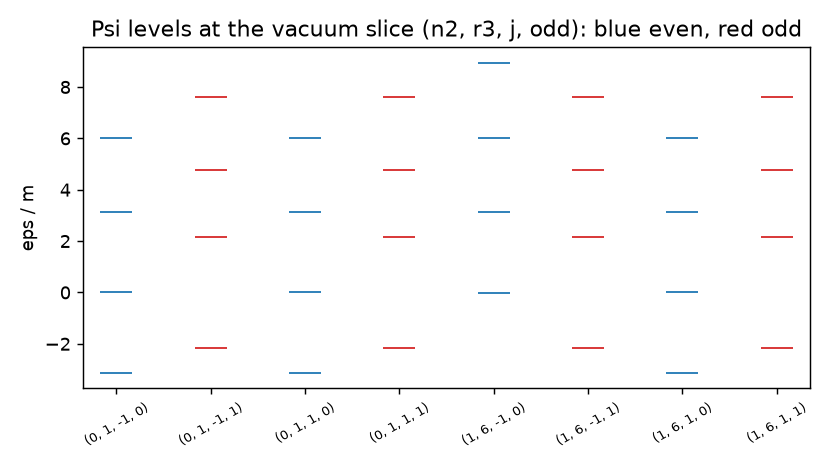
\includegraphics[width=0.85\linewidth]{solution/figures/fig6_psi_levels.png}
\caption{Levels of Psi at the vacuum slice by sector (n2, r3, j, odd).}
\end{figure}

\subsection*{5.3 Coupling to the Standard Model: linear response}
\addcontentsline{toc}{subsection}{5.3 Coupling to the Standard Model: linear response}

Ground states $N = 8$ (the fold zero modes) and $N = 592$ (a fold-band gas) are computed for $\lambda = 0$ and for $\lambda_1$ of the record (157.7 and 2.131). For each portal the solver gives the following (table in section 9):
\begin{itemize}
\item the Hellmann-Feynman check: $dE_{KS}/de$ from Richardson differences at fixed occupations equals $\int(\partial M/\partial e\,S + \partial v/\partial e\,n)$ (check K4). The scalar portals do not act on the chiral zero modes at $\lambda = 0$, whose scalar density vanishes; these are null cases.
\item the y-exchange identity at $e = 0.02$ (check K5), the conservation law of the hidden direction with the force of the external field:
\end{itemize}
\[\adjustbox{max width=\linewidth}{$\displaystyle \big[e^{3Hy}p_0\big]_{-L}^{0} - 3H\int e^{3Hy}p_t\,dy = -\int e^{3Hy}\big(M_{ext}'S + v_{ext}'n\big)\,dy ,$}\]
satisfied to $O(h^2)$.
\begin{itemize}
\item the response of the dark-matter level, of the fold band and of the sources.
\end{itemize}

The fold band stays massless. Without the self-interaction its gap at the lowest shell changes by less than $10^{-14}$ per unit $e$, and the vector portal shifts all fold levels together (a chemical-potential shift). With $\lambda_1$ the vector portal changes it by $-4.0\times10^{-7}$ per unit $e$, a second-order mean-field effect of no consequence for portal amplitudes of physical size. The dark-matter level moves linearly with every portal; this is the dark-matter–Standard-Model interaction of the model in the mean-field limit.

\subsection*{5.4 Cold dark matter}
\addcontentsline{toc}{subsection}{5.4 Cold dark matter}

Eight dark-matter quanta are placed in the lowest odd levels ($k = 0$, $j = \pm1$) on top of the $N = 8$ ground state, with fixed occupations and solved self-consistently on three grids. The added energy-momentum is cold: $w = p_3/\rho = 0$ at $\lambda = 0$ (check K6). It has a hidden pressure $p_0/\rho$ (section 9), which pushes on the block through $\delta k = \kappa p_0/(3H^2)$.

\subsection*{5.5 The coupled fixed point}
\addcontentsline{toc}{subsection}{5.5 The coupled fixed point}

The loop runs as follows:
\begin{enumerate}
\item the Kohn-Sham state with the vector portal of the electron density;
\item its x0-averaged hidden pressure $\bar p_0$;
\item the block shift $\delta k = \sigma\bar p_0/3$, with $\sigma = \kappa/H^2$ in the units of the Kohn-Sham densities;
\item the new $f = (k_0 + \delta k)^{-1/2}$ and the new $c_f = f\mu_fL$ and $m_{KK} \propto 1/f$;
\item the new portal profile and the new Standard-Model masses;
\item the Kohn-Sham state again.
\end{enumerate}

It converges for $\sigma = 10^{-3}$ and $10^{-1}$ (check K7). The resulting shifts of $f$ and of the masses are in section 9. At late times $\sigma\bar p_0$ is of order $(A/H)^2$, so the feedback is of order $10^{-93}$. The coupling of $\Psi$ to all other fields matters in the primordial era, which is the subject of the record's phases W5 to W8.

\section*{6. CMB, CNB and BAO}
\addcontentsline{toc}{section}{6. CMB, CNB and BAO}

The late universe is the four-dimensional effective theory of the vacuum with $G_{eff} = G$ (benchmark). Its components are:
\begin{itemize}
\item photons ($T_{CMB} = 2.7255$ K);
\item one neutrino species ($N_{eff,SM} = 3.044/3 = 1.0147$, $m_\nu = 0.05$ eV);
\item the $\Psi$ fold band (massless, $g_F = 8$, decoupled at $T_{dec}$);
\item the $\Psi$ dark matter ($\omega_c = 0.1200$, set by the relic density);
\item baryons from $u$ and $d$ by QCD ($\omega_b = 0.02237$);
\item $\delta\Lambda$, for flatness.
\item $\Delta N_{eff} = (g_F/2)(T_\Psi/T_\nu)^4$ with $(T_\Psi/T_\nu)^3 = 7.25/g_{*s}(T_{dec})$. Here $g_{*s}$ counts the UM-1 content: one generation and no Higgs, so it is 53.25 above $m_W$, 44.25 down to the QCD crossover, 10.25 in the pion gas and 7.25 below 20 MeV.
\item Fitting formulae: Hu-Sugiyama $z_*$ and Eisenstein-Hu $z_{drag}$; the sound horizon is a numerical integral. They are calibrated once on Planck 2018 $\Lambda$CDM (the factors 1.00198 on $\theta_*$ and 0.97684 on $r_{drag}$). $h$ is fitted to $100\theta_* = 1.04110$.
\item The first peak uses $\ell_1 = \ell_A(1 - \phi_1)$ with $\phi_1 = 0.267(r_*/0.3)^{0.1}$.
\item BAO: the eBOSS DR16 BAO-only consensus, 12 measurements from $z = 0.15$ to $2.33$.
\end{itemize}

Results (section 9):
\begin{itemize}
\item Decoupling above the QCD crossover gives $N_{eff} = 1.30$ to $1.37$, excluded at about $10\sigma$. It also forces $H_0 \approx 48$ km/s/Mpc at fixed $\theta_*$ and $\omega$'s, and BAO $\chi^2 > 600$.
\item Pion-gas decoupling gives $N_{eff} = 3.54$ ($+3.2\sigma$, BAO $\chi^2 = 33.8$). Decoupling below 20 MeV gives 5.02.
\item $N_{eff} = 2.99$ requires $g_{*s}(T_{dec}) = 12.31$: $\Psi$ must decouple inside the QCD crossover (about 150 MeV). Then $H_0 = 66.75$ km/s/Mpc, $r_{drag} = 147.39$ Mpc, $\ell_A = 301.76$ (fixed by the fit of $\theta_*$), $\ell_1 = 220.7$, and BAO $\chi^2 = 11.6$ for 12 points.
\item This is the model's sharpest cosmological prediction: the dirac16complex fold band must stand in for the two missing neutrino species, and its decoupling temperature is fixed to the QCD crossover. With the 4D portal scale this sets $G_V^{-1/2} \approx 13$ TeV (a neutrino-like decoupling estimate, STANDARD).
\item CNB: $T_\nu = 1.9454$ K and $n_\nu = 112$ cm$^{-3}$ for the one species. The $\Psi$ fold background has $T_\Psi = 1.63$ K and $n_\Psi = 264$ cm$^{-3}$ (section 9). Both are relativistic today except the massive $\nu$ ($m_\nu \gg T_\nu$).
\end{itemize}

\begin{figure}[htbp]
\centering
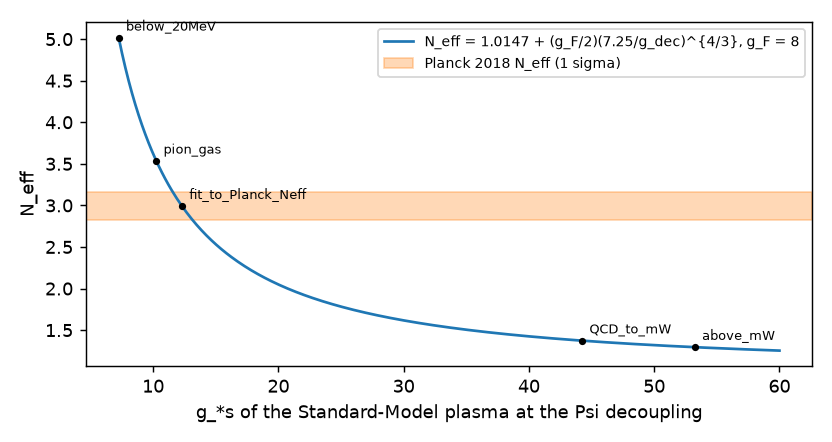
\includegraphics[width=0.85\linewidth]{solution/figures/fig4_neff.png}
\caption{N\_eff against g\_*s at the Psi decoupling, with the Planck band and the scenarios.}
\end{figure}

\begin{figure}[htbp]
\centering
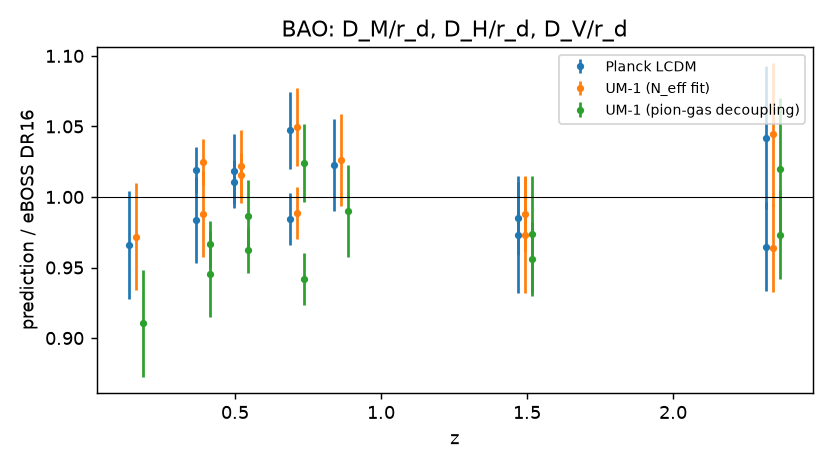
\includegraphics[width=0.85\linewidth]{solution/figures/fig5_bao.png}
\caption{BAO predictions over eBOSS DR16 data for Planck LCDM and two UM-1 scenarios.}
\end{figure}

\section*{7. Assumptions, changes, conflicts and open problems}
\addcontentsline{toc}{section}{7. Assumptions, changes, conflicts and open problems}

\begin{itemize}
\item CHANGED: $w_3 = 1/768$ (author: 1/1152) and $\Lambda = -24H^2 + \delta\Lambda$ (author: $-10H^2$). The author's values give repulsive four-dimensional gravity in the only static vacuum (section 3.2).
\item ASSUMED:
\begin{itemize}
\item a block stabiliser with curvature above $2H^2$ (section 3.3);
\item the exact fold-reflection parity that keeps the dark matter stable;
\item $m = H$ for $\Psi$ (the record's units);
\item $\lambda_f = 1$ and $c_L = c_R$ for the fermions;
\item $m_\nu = 0.05$ eV;
\item the fermion profile shapes of the portal fields;
\item Planck's $\omega_b$ and $\omega_c$ as inputs.
\end{itemize}
\item LABELLED DEPARTURE: in the late era the extra times deflate at the rate $h_4 \approx -10^{-93}A$ (section 3.4), not exponentially. They are never static.
\item CONFLICTS WITH DATA:
\begin{itemize}
\item No Higgs, while a 125 GeV Higgs boson is observed. Without it, the longitudinal $WW$ amplitude grows like $s/v^2$ and violates unitarity near $\sqrt{8\pi}\,v \approx 1.2$ TeV, while the KK modes that could restore it lie at 121 TeV.
\item The S parameter of the Higgsless tip is not computed (OPEN).
\item One generation makes $N_{eff}$ fit only for a decoupling inside the QCD crossover.
\item The cosmological term needs $\delta\Lambda/H^2 \approx 7.5\times10^{-93}$ (the cosmological-constant problem, unsolved here).
\end{itemize}
\item OPEN:
\begin{itemize}
\item the stabiliser (the Casimir energy of the cell);
\item the reduction of the Psi self-interaction to the relic cross-section;
\item the portal coefficients;
\item the primordial-era solution (the W phases of the Revision record);
\item the order-$\epsilon$ Lovelock corrections to the perturbations (only the effective Newton constant is used);
\item BBN with $N_{eff}(T)$;
\item the CMB damping tail, which needs a recombination code.
\end{itemize}
\end{itemize}

\section*{8. Reproduction}
\addcontentsline{toc}{section}{8. Reproduction}

From \texttt{Revision/\allowbreak{}universe\_\allowbreak{}model/\allowbreak{}solution} (every calculation under \texttt{timeout -{}\allowbreak{}k 5 423}):

\begin{Verbatim}[fontsize=\small]
python ks_coupled.py spectrum         # 4 s
python ks_coupled.py portal8_lam0     # 50 s
python ks_coupled.py portal8_lam1     # 141 s
python ks_coupled.py portal592_lam0   # 53 s
python ks_coupled.py portal592_lam1   # 158 s
python ks_coupled.py dm_lam0          # 60 s
python ks_coupled.py dm_lam1          # 107 s
python ks_coupled.py loop             # 50 s
python solve_model.py                 # 35 s: vacua, masses, cosmology,
                                      # figures, checks, the tables below
\end{Verbatim}

The PDF is built from the repository root with \texttt{bash Revision/\allowbreak{}universe\_\allowbreak{}model/\allowbreak{}tools/\allowbreak{}build\_\allowbreak{}pdfs.\allowbreak{}sh SOLUTION}.

\section*{9. Results}
\addcontentsline{toc}{section}{9. Results}


\subsection*{9.1 Generated tables (from \texttt{solution/\allowbreak{}solve\_\allowbreak{}model.\allowbreak{}py}; every number below is from the run)}
\addcontentsline{toc}{subsection}{9.1 Generated tables (from \texttt{solution/\allowbreak{}solve\_\allowbreak{}model.\allowbreak{}py}; every number below is from the run)}

\textbf{Vacuum and block (vacua.py).}

\begin{longtable}{>{\raggedright\arraybackslash}p{0.152\linewidth}>{\raggedright\arraybackslash}p{0.055\linewidth}>{\raggedright\arraybackslash}p{0.097\linewidth}>{\raggedright\arraybackslash}p{0.097\linewidth}>{\raggedright\arraybackslash}p{0.161\linewidth}>{\raggedright\arraybackslash}p{0.256\linewidth}}
\toprule
\textbf{weights $w$} & \textbf{$k_0$} & \textbf{$\Lambda_0/H^2$} & \textbf{$G(k_0)$} & \textbf{4D gravity} & \textbf{block mode $\lambda^2/H^2$} \\
\midrule
{}(1, 1/32, 1/1152) & 8 & -24 & -1 & repulsive & -2 (stable (oscillatory)) \\
{}(1, 1/32, 1/768) & 8 & -24 & 1 & attractive & 2 (unstable (real eigenvalue)) \\
\bottomrule
\end{longtable}

\textbf{Mass spectrum (masses.py; $\eta = HL = 3$, $f = k_0^{-1/2}$).}

\begin{longtable}{>{\raggedright\arraybackslash}p{0.521\linewidth}>{\raggedright\arraybackslash}p{0.365\linewidth}}
\toprule
\textbf{quantity} & \textbf{value} \\
\midrule
$m_{KK}$ (first photon/gluon/graviton KK level, fitted to $\rho_0 - 1$) & $1.212 \times 10^{5}$ GeV \\
$H$ & $23421$ GeV \\
proper half-cell $fL$ & $8.936 \times 10^{-21}$ m \\
period of $x_0$, $\pi/(6H)$ & $2.236 \times 10^{-5}$ GeV$^{-1}$ = $4.411 \times 10^{-21}$ m \\
largest $m_W$ of a positive tip term & $0.01824\, m_{KK}$ (so $m_{KK} \geq 4407$ GeV) \\
$\beta_W$, $\beta_Z$ (tip Robin parameters) & $0.01194$, $0.01537$ \\
$m_Z$ predicted (from $m_W$, on-shell $\cos^2\theta_W$) & $91.17068$ GeV (observed 91.188; difference $-0.01732$ GeV) \\
$\rho - 1$ (tree) & $3.800 \times 10^{-4}$ \\
W: bulk hidden-momentum part / tip part of $m_W^2$ & $0.001322$ / $0.9987$ \\
first W KK level & $1.212 \times 10^{5}$ GeV \\
photon, gluon, graviton & $\Lambda_0 = 0$: massless \\
\bottomrule
\end{longtable}

\begin{longtable}{>{\raggedright\arraybackslash}p{0.165\linewidth}>{\raggedright\arraybackslash}p{0.190\linewidth}>{\raggedright\arraybackslash}p{0.213\linewidth}>{\raggedright\arraybackslash}p{0.151\linewidth}>{\raggedright\arraybackslash}p{0.116\linewidth}}
\toprule
\textbf{fermion} & \textbf{$m_f$ (GeV)} & \textbf{$m_f/m_{KK} = \zeta(c_f)^2$} & \textbf{$c_f = f\mu_f L$} & \textbf{$\mu_f/H$} \\
\midrule
nu & $5.000 \times 10^{-11}$ & $4.126 \times 10^{-16}$ & 19.54 & 18.43 \\
e & $5.110 \times 10^{-4}$ & $4.217 \times 10^{-9}$ & 11.2 & 10.56 \\
u & $0.00216$ & $1.782 \times 10^{-8}$ & 10.44 & 9.844 \\
d & $0.0047$ & $3.878 \times 10^{-8}$ & 10.03 & 9.458 \\
\bottomrule
\end{longtable}

\begin{longtable}{>{\raggedright\arraybackslash}p{0.143\linewidth}>{\raggedright\arraybackslash}p{0.140\linewidth}>{\raggedright\arraybackslash}p{0.129\linewidth}>{\raggedright\arraybackslash}p{0.157\linewidth}>{\raggedright\arraybackslash}p{0.265\linewidth}}
\toprule
\textbf{fermion} & \textbf{width $\Delta t$} & \textbf{$\Delta s$ (m)} & \textbf{$\hbar c/(2\Delta s)$ (GeV)} & \textbf{$m_f$ / Heisenberg estimate} \\
\midrule
nu & 0.02558 & $2.286 \times 10^{-22}$ & $4.316 \times 10^{5}$ & $1.159 \times 10^{-16}$ \\
e & 0.04466 & $3.991 \times 10^{-22}$ & $2.472 \times 10^{5}$ & $2.067 \times 10^{-9}$ \\
u & 0.04789 & $4.280 \times 10^{-22}$ & $2.305 \times 10^{5}$ & $9.369 \times 10^{-9}$ \\
d & 0.04984 & $4.454 \times 10^{-22}$ & $2.215 \times 10^{5}$ & $2.122 \times 10^{-8}$ \\
\bottomrule
\end{longtable}

\textbf{dirac16complex, Kohn-Sham (ks\_coupled.py; units $m = H$).}

\begin{longtable}{>{\raggedright\arraybackslash}p{0.469\linewidth}>{\raggedright\arraybackslash}p{0.417\linewidth}}
\toprule
\textbf{quantity} & \textbf{value} \\
\midrule
vacuum slice $a_{4} = 3\ln 8/2$, $f$, $\kappa = e^{-a_4}$ & 3.119, 0.3536, 0.04419 \\
fold zero modes; fold band & 8 at $k = 0$; $\varepsilon = \kappa|k|$ exactly (massless), $g_F = 8$ \\
lowest odd bulk level (dark matter) & $2.17492\,m$ = $50939$ GeV \\
lowest even bulk level & $3.126177\,m$ \\
dark matter ($\lambda$ = 0): energy per 8 quanta, $w = p_3/\rho$, $p_0/\rho$ & $17.39936$, $0$, $0.6575$ \\
dark matter ($\lambda$ = 157.7): energy per 8 quanta, $w = p_3/\rho$, $p_0/\rho$ & $17.4307$, $0.001817$, $0.6567$ \\
\bottomrule
\end{longtable}

\begin{longtable}{>{\raggedright\arraybackslash}p{0.111\linewidth}>{\raggedright\arraybackslash}p{0.107\linewidth}>{\raggedright\arraybackslash}p{0.129\linewidth}>{\raggedright\arraybackslash}p{0.282\linewidth}>{\raggedright\arraybackslash}p{0.205\linewidth}}
\toprule
\textbf{state (grid 600)} & \textbf{portal} & \textbf{$dE_{KS}/de$} & \textbf{Hellmann-Feynman deviation} & \textbf{y-exchange residual ($e = 0.02$)} \\
\midrule
N = 8, $\lambda$ = 0 & eD & 0 & null (both zero) & null (all terms zero) \\
N = 8, $\lambda$ = 0 & eS & 0 & null (both zero) & null (all terms zero) \\
N = 8, $\lambda$ = 0 & eV & $0.7865$ & $2.259 \times 10^{-14}$ & $7.609 \times 10^{-5}$ \\
N = 8, $\lambda$ = 157.7 & eD & $4.689 \times 10^{-5}$ & $3.690 \times 10^{-10}$ & $1.700 \times 10^{-6}$ \\
N = 8, $\lambda$ = 157.7 & eS & $4.656 \times 10^{-4}$ & $5.677 \times 10^{-11}$ & $2.986 \times 10^{-7}$ \\
N = 8, $\lambda$ = 157.7 & eV & $0.7865$ & $2.856 \times 10^{-13}$ & $7.149 \times 10^{-5}$ \\
N = 592, $\lambda$ = 0 & eD & 0 & null (both zero) & null (all terms zero) \\
N = 592, $\lambda$ = 0 & eS & 0 & null (both zero) & null (all terms zero) \\
N = 592, $\lambda$ = 0 & eV & $58.2$ & $1.343 \times 10^{-15}$ & $7.609 \times 10^{-5}$ \\
N = 592, $\lambda$ = 2.131 & eD & $0.00347$ & $8.071 \times 10^{-10}$ & $1.701 \times 10^{-6}$ \\
N = 592, $\lambda$ = 2.131 & eS & $0.03446$ & $1.731 \times 10^{-10}$ & $2.985 \times 10^{-7}$ \\
N = 592, $\lambda$ = 2.131 & eV & $58.2$ & $2.998 \times 10^{-13}$ & $7.149 \times 10^{-5}$ \\
\bottomrule
\end{longtable}

\begin{longtable}{>{\raggedright\arraybackslash}p{0.182\linewidth}>{\raggedright\arraybackslash}p{0.133\linewidth}>{\raggedright\arraybackslash}p{0.155\linewidth}>{\raggedright\arraybackslash}p{0.208\linewidth}>{\raggedright\arraybackslash}p{0.157\linewidth}}
\toprule
\textbf{state (grid 600)} & \textbf{portal} & \textbf{$d\varepsilon_{DM}/de$} & \textbf{$d(\varepsilon_{n2=1} - \varepsilon_0)/de$} & \textbf{$d\bar p_0/de$} \\
\midrule
N = 8, $\lambda$ = 0 & eD & $0.006409$ & below $10^{-14}$ & 0 \\
N = 8, $\lambda$ = 0 & eS & $0.03543$ & below $10^{-14}$ & 0 \\
N = 8, $\lambda$ = 0 & eV & $0.03231$ & below $10^{-14}$ & $-2.564 \times 10^{-7}$ \\
N = 8, $\lambda$ = 157.7 & eD & $0.006414$ & $8.262 \times 10^{-11}$ & $3.432 \times 10^{-11}$ \\
N = 8, $\lambda$ = 157.7 & eS & $0.03571$ & $1.947 \times 10^{-9}$ & $6.440 \times 10^{-10}$ \\
N = 8, $\lambda$ = 157.7 & eV & $0.03266$ & $-3.968 \times 10^{-7}$ & $-2.564 \times 10^{-7}$ \\
N = 592, $\lambda$ = 0 & eD & $0.006409$ & below $10^{-14}$ & 0 \\
N = 592, $\lambda$ = 0 & eS & $0.03543$ & below $10^{-14}$ & 0 \\
N = 592, $\lambda$ = 0 & eV & $0.03231$ & below $10^{-14}$ & $-1.898 \times 10^{-5}$ \\
N = 592, $\lambda$ = 2.131 & eD & $0.006414$ & $8.262 \times 10^{-11}$ & $2.540 \times 10^{-9}$ \\
N = 592, $\lambda$ = 2.131 & eS & $0.03571$ & $1.947 \times 10^{-9}$ & $4.766 \times 10^{-8}$ \\
N = 592, $\lambda$ = 2.131 & eV & $0.03266$ & $-3.968 \times 10^{-7}$ & $-1.898 \times 10^{-5}$ \\
\bottomrule
\end{longtable}

\begin{longtable}{>{\raggedright\arraybackslash}p{0.165\linewidth}>{\raggedright\arraybackslash}p{0.181\linewidth}>{\raggedright\arraybackslash}p{0.122\linewidth}>{\raggedright\arraybackslash}p{0.107\linewidth}>{\raggedright\arraybackslash}p{0.122\linewidth}>{\raggedright\arraybackslash}p{0.122\linewidth}}
\toprule
\textbf{coupled fixed point} & \textbf{iterations} & \textbf{$\delta k$} & \textbf{$\delta f/f$} & \textbf{$\delta m_e/m_e$} & \textbf{$\delta m_\nu/m_\nu$} \\
\midrule
$\sigma$ = 0.001 & 2 & $-1.617 \times 10^{-10}$ & $1.011 \times 10^{-11}$ & $-2.263 \times 10^{-10}$ & $-3.950 \times 10^{-10}$ \\
$\sigma$ = 0.1 & 2 & $-1.617 \times 10^{-8}$ & $1.011 \times 10^{-9}$ & $-2.263 \times 10^{-8}$ & $-3.950 \times 10^{-8}$ \\
\bottomrule
\end{longtable}

\textbf{Cosmology (cosmology.py).}

\begin{longtable}{>{\raggedright\arraybackslash}p{0.168\linewidth}>{\raggedright\arraybackslash}p{0.168\linewidth}>{\raggedright\arraybackslash}p{0.079\linewidth}>{\raggedright\arraybackslash}p{0.110\linewidth}>{\raggedright\arraybackslash}p{0.165\linewidth}>{\raggedright\arraybackslash}p{0.128\linewidth}}
\toprule
\textbf{model} & \textbf{$g_{*s}$ at decoupling} & \textbf{$N_{eff}$} & \textbf{pull vs Planck} & \textbf{$H_0$ (km/s/Mpc)} & \textbf{BAO $\chi^2$ (12 points)} \\
\midrule
Planck LCDM (reference) & - & 3.046 & - & 67.36 & 10.25 \\
UM-1, above mW & 53.25 & 1.295 & -9.97 & 47.33 & 680.7 \\
UM-1, QCD to mW & 44.25 & 1.373 & -9.51 & 48.22 & 614 \\
UM-1, pion gas & 10.25 & 3.536 & 3.21 & 73.11 & 33.77 \\
UM-1, below 20MeV & 7.25 & 5.015 & 11.9 & 90.63 & 390 \\
UM-1, fit to Planck Neff & 12.31 & 2.99 & 0 & 66.75 & 11.64 \\
\bottomrule
\end{longtable}

\begin{longtable}{>{\raggedright\arraybackslash}p{0.242\linewidth}>{\raggedright\arraybackslash}p{0.109\linewidth}>{\raggedright\arraybackslash}p{0.126\linewidth}>{\raggedright\arraybackslash}p{0.134\linewidth}>{\raggedright\arraybackslash}p{0.109\linewidth}>{\raggedright\arraybackslash}p{0.097\linewidth}}
\toprule
\textbf{model} & \textbf{$100\theta_*$} & \textbf{$z_*$} & \textbf{$r_{drag}$ (Mpc)} & \textbf{$\ell_A$} & \textbf{$\ell_1$} \\
\midrule
Planck LCDM (reference) & 1.0411 & 1091.85 & 147.09 & 301.76 & 220.7 \\
UM-1, above mW & 1.0411 & 1091.85 & 156.69 & 301.76 & 222.8 \\
UM-1, QCD to mW & 1.0411 & 1091.85 & 156.21 & 301.76 & 222.7 \\
UM-1, pion gas & 1.0411 & 1091.85 & 144.79 & 301.76 & 220.2 \\
UM-1, below 20MeV & 1.0411 & 1091.85 & 138.48 & 301.76 & 218.7 \\
UM-1, fit to Planck Neff & 1.0411 & 1091.85 & 147.39 & 301.76 & 220.7 \\
\bottomrule
\end{longtable}

\begin{longtable}{>{\raggedright\arraybackslash}p{0.600\linewidth}>{\raggedright\arraybackslash}p{0.286\linewidth}}
\toprule
\textbf{background today} & \textbf{value} \\
\midrule
$T_\nu = (4/11)^{1/3}T_{CMB}$ & 1.9454 K \\
$n_\nu$ (one species, $\nu + \bar\nu$) & 112 cm$^{-3}$ \\
$T_\Psi$ of the fold band (N\_eff fit) & 1.631 K \\
$n_\Psi$ of the fold band ($g_F = 8$) & 264 cm$^{-3}$ \\
$(H_0/H)^2$ & $3.696 \times 10^{-93}$ \\
deflation today $h_4/\dot a_4$ & $-8.857 \times 10^{-94}$ \\
$\delta\Lambda/H^2$ (dark energy) & $7.545 \times 10^{-93}$ \\
\bottomrule
\end{longtable}

\textbf{Checks} (\texttt{solution/\allowbreak{}reports/\allowbreak{}solution-{}\allowbreak{}checks.\allowbreak{}json}, 21 of 21 PASS): V1, V2, V3, V4, M1, M2, M3, M4, M5, M6, M7, K1, K2, K3, K4, K5, K6, K7, C1, C2, C3.


\end{document}
